\hypertarget{_solution_analysis_8cpp}{}\section{/home/zheng/catkin\+\_\+ws/src/qp\+O\+A\+S\+E\+S-\/3.2.1/src/\+Solution\+Analysis.cpp File Reference}
\label{_solution_analysis_8cpp}\index{/home/zheng/catkin\+\_\+ws/src/qp\+O\+A\+S\+E\+S-\/3.\+2.\+1/src/\+Solution\+Analysis.\+cpp@{/home/zheng/catkin\+\_\+ws/src/qp\+O\+A\+S\+E\+S-\/3.\+2.\+1/src/\+Solution\+Analysis.\+cpp}}
{\ttfamily \#include $<$qp\+O\+A\+S\+E\+S/extras/\+Solution\+Analysis.\+hpp$>$}\newline
Include dependency graph for Solution\+Analysis.\+cpp\+:
\nopagebreak
\begin{figure}[H]
\begin{center}
\leavevmode
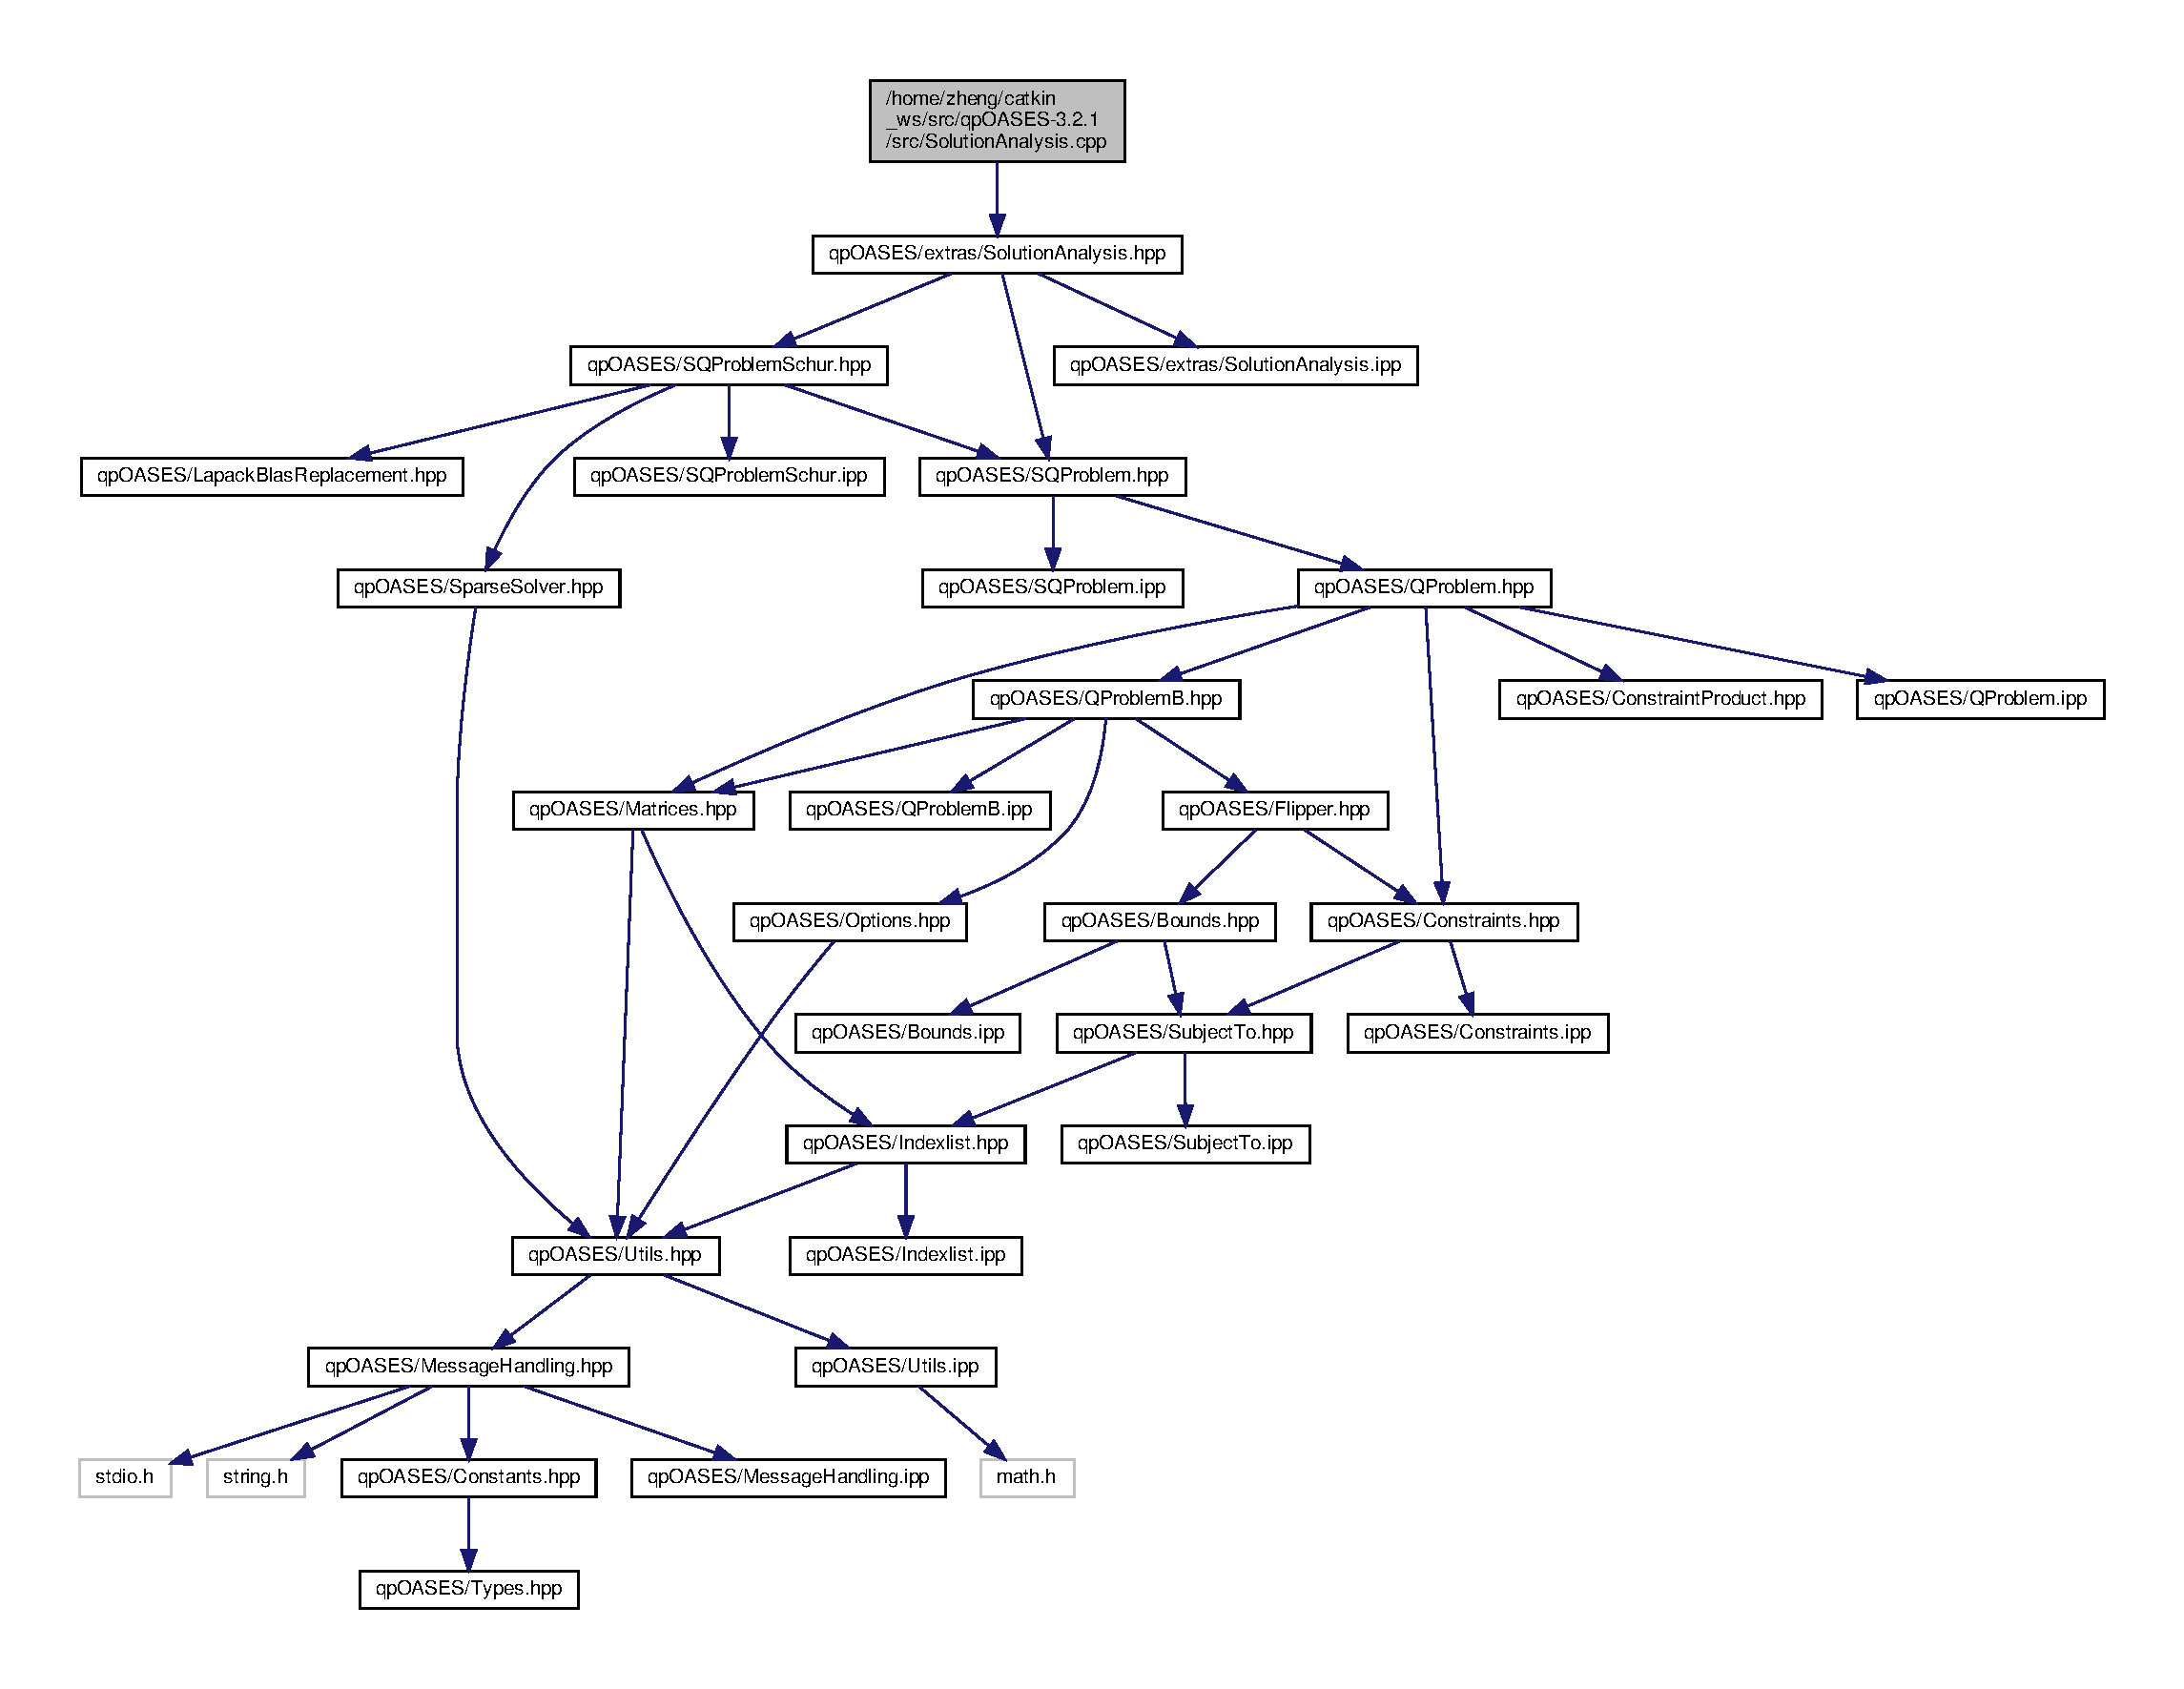
\includegraphics[width=350pt]{_solution_analysis_8cpp__incl}
\end{center}
\end{figure}


\subsection{Detailed Description}
\begin{DoxyAuthor}{Author}
Hans Joachim Ferreau (thanks to Boris Houska) 
\end{DoxyAuthor}
\begin{DoxyVersion}{Version}
3.\+2 
\end{DoxyVersion}
\begin{DoxyDate}{Date}
2008-\/2017
\end{DoxyDate}
Implementation of the \hyperlink{class_solution_analysis}{Solution\+Analysis} class designed to perform additional analysis after solving a QP with qp\+O\+A\+S\+ES. 